\documentclass{include/tfgitic}[2022/06/30]

%\usepackage{}

\addbibresource{misc/tfg.bib}

\title{Implementació d'una pantalla inte\l.ligent}
\subtitle{Creació d'un dispositiu i programari que actualitzi l'orientació
          d'una pantalla al rotar-la}

\author{Eric Roy Almonacid}
\advisor{Francisco del Águila López}

\dedication{Per l'avi, que hagués sigut el primer comprador d'aquest producte}

\begin{acknowledgments}
    Aquest treball no hagués existit si no fos per l'Isaac Iglesias, que em va
    proposar fer aquest projecte, i a poc a poc ha vist com la seva idea anava
    convertint-se en un producte.

    Una altra persona a qui dec aquest treball és al meu tutor del projecte, el
    Francisco del Águila, que m'ha orientat i recolzat durant tot aquest procés.

    També voldria agrair al professorat de l'EPSEM, però en especial al Joan
    Martínez que, juntamtent amb el meu tutor, m'ha aconsellat durant el disseny
    de la placa de circuit imprès.

    Finalment, vull donar les gràcies a totes les persones del meu entorn
    quotidià que, potser fins i tot sense ells saber-ho, han fet que aquests
    mesos no semblin tan durs. Familiars, amics, companys de feina i d'estudis,
    aquest treball també és vostre.
\end{acknowledgments}

\begin{resum}
    La tendència a generar contingut audiovisual en format vertical és una de
    les diverses causes per la qual la gent es plantegi tenir una pantalla de
    l'ordinador en aquesta nova orientació. 
    Una de les solucions més senzilles i econòmiques és adquirir un suport de
    monitor que permeti rotar la pantalla sense haver-la de desmuntar, i així
    disposar fàcilment de les dues orientacions.

    Un inconvenient d'aquest sistema és que, quan es gira la pantalla, s'ha de
    reconfigurar l'entorn gràfic per adaptar-lo a la nova orientació.
    Existeixen alguns monitors d'alta gamma que, mitjançant la connexió d'imatge
    ja existent, poden notificar l'ordinador els canvis d'orientació. Tanmateix,
    aquests sistemes només funcionen correctament si s'utilitza el suport de
    pantalla i protocols recomanats.

    Aquest projecte proposa un dispositiu de baix cost que, mitjançant un sensor
    giroscòpic i una connexió USB, detecta l'orientació de la pantalla i
    configura l'entorn gràfic adequadament. S'ha posat èmfasi en l'ús de
    protocols estàndards existents, la compatibilitat entre diferents sistemes
    operatius i la facilitat d'insta\l.lació i ús dels programes relacionats
    amb el dispositiu.
\end{resum}

\begin{abstract}
    The trend towards generating audiovisual content in vertical format is one
    of the various reasons why people consider having a computer screen in this
    new orientation.
    One of the simplest and most economical solutions is to acquire a monitor
    stand that allows the screen to be rotated without having to disassemble it,
    thus easily providing both orientations.

    One drawback of this system is that when the screen is rotated, the graphic
    environment needs to be reconfigured to adapt to the new orientation.
    There are some high-end monitors that, through the existing image
    connection, can notify the computer of orientation changes. However,
    these systems only work properly if the recommended screen support and
    protocols are used.

    This project proposes a low-cost device that, using a gyroscope sensor and a
    USB connection, detects the screen orientation and configures the graphic
    environment accordingly. Emphasis has been placed on the use of existing
    standard protocols, compatibility between different operating systems, and
    the ease of installation and use of device-related programs.
\end{abstract}

\begin{document}

%\part{Memòria}

\chapter{Introducció}
\label{cap:introduccio}

Durant els darrers anys, el contingut digital en format vertical no ha cessat
d'augmentar, sent una de les principals causes l'ús generalitzat dels
dispositius mòbils \cite{Navarro2023El}. Les xarxes socials no van tardar a
adaptar les seves interfícies a aquestes noves resolucions. De fet, aquesta
tendència també s'ha portat a moltes altres aplicacions, tan de mòbil com
d'escriptori. Per exemple, han nascut termes com el
\est{Mobile-First Web Design}, que incita als desenvolupadors de pàgines web
a dissenyar les pàgines per a dispositius mòbils, i adaptar-les després
(el contrari del que es feia tradicionalment) \cite{varrela2015mobile}.

Tot plegat ha creat una nova moda: tenir una pantalla en vertical
en un ordinador de sobretaula. La majoria de monitors es poden muntar en
aquesta orientació sense necessitar un altre suport, pel que aquesta pràctica
s'ha popularitzat molt fàcilment \cite{WeardenPortrait}.
Disposar d'una pentalla en vertical també pot aportar altres avantatges. Per
exemple: els desenvolupadors poden veure més línies d'un mateix fitxer de codi
a la vegada, els dissenyadors de cartells o continguts per a dispositius mòbils
també poden beneficiar-se d'aquesta orientació.

Tanmateix, de vegades pot resultar més útil veure contingut en format
horizontal, com per exemple les pe\l.lícules. Si disposem de la configuració
anterior, hauríem de desmuntar la pantalla del suport i tornar-la a co\l.locar
en l'orientació desitjada. Un cop fet això, s'hauria d'anar a la configuració
del sistema per a que l'entorn gràfic del sistema operatiu mostri els continguts
d'aquella pantalla correctament. Aquest cúmul de tasques fan aquest procediment
tediós, sent aquest un motiu pel que no es sol dur a terme.

Per a resoldre aquest problema, han sortit a la venda suports rotatoris per a 
monitors \cite{DIGITUSUniversal}. Aquests redueixen el problema mencionat
anteriorment a només haver de girar la pantalla amb la força de la mà, i
configurar l'entorn gràfic. Algunes marques han anat més enllà, oferint
monitors incorporats amb un sensor de gravetat que, al detectar un canvi
d'orientació s'encarreguen d'actualitzar l'entorn gràfic \cite{LCLC}.

Malauradament, aquests últims tipus de productes tenen alguns punts negatius:
\begin{itemize}
    \item El fabricant només assegura que s'actualitzi l'orientació en l'entorn
    gràfic si el sistema operatiu és Windows.
    \item Aquest sistema d'actualització funciona per sobre del protocol de
    transmissió de l'imatge (en aquest cas, \acro{hdmi}), i no es garanteix el correcte
    funcionament en altres connexions.
    \item Finalment, s'ha de comprar una nova pantalla per a poder gaudir del
    sistema. És a dir, el fabricant no ven per separat un dispositiu que tingués
    el mateix propòsit i pugués allargar la vida útil d'una pantalla ja
    comprada.
\end{itemize}

Així doncs, l'objectiu principal d'aquest treball és crear un dispositiu que,
juntament amb un suport rotatori ja existent, pugui convertir la tasca de girar
el monitor en un gest habitual durant una rutina de treball. Es posarà èmfasi en
la facilitat d'insta\l.lació i ús, compatibilitat amb diferents sistemes
operatius, i a una hipotètica comercialització del producte.

La motivació darrera l'elecció d'aquest treball rau en l'interès personal en
posar en pràctica totes les àrees de coneixement que composen la titulació que
s'està cursant. Adicionalment, també hi havia un interès personal per a obtenir
un producte final que pot aportar un ús en el dia a dia. Per aquest motiu, quan
es va presentar l'oportunitat de dissenyar el producte mencionat anteriorment,
es va pensar que era una molt bona manera per a donar un final rodó al grau.

\chapter{Objectius}
\label{cap:objectius}

\section{Objectius generals}

L'objectiu principal d'aquest treball de fi de grau és implementar un dispositiu
de dimensions reduïdes, que s'enganxarà darrere el monitor i es connectarà
a l'ordinador mitjançant un cable \acro{usb}. Aquest dispositiu contindrà els
sensors i altres components necessaris per poder informar l'ordinador sobre
l'orientació actual de la pantalla. A través d'un programari propi i de la
interfície de programació que proporciona l'entorn gràfic, es canviarà
l'orientació de la pantalla en funció de les dades rebudes del dispositiu. Es
buscarà sempre la màxima compatibilitat possible, facilitat d'insta\l.lació i
ús quotidià, i un preu de construcció raonable.


\section{Objectius específics}

Aquest treball de fi de grau es podria extendre molt més enllà dels pocs mesos
de temps dels que es disposa. Per això, es definiran uns objectius essencials
per considerar el projecte completat, i uns objectius addicionals o
ampliacions que, tot i no ser troncals pel projete, poden completar o
millorar el sistema.

Objectius essencials:
\begin{itemize}
    \item Fer una recerca sobre la tecnologia i pràctiques actuals sobre el 
    procés de disseny de dispositius \acro{usb}.
    \item Escollir els components electrònics del dispositiu i dissenyar una
    placa de circuit imprès. S'imprimiran unes quantes plaques per poder fer
    proves del sistema complet.
    \item Definir la forma en què l'usuari podrà insta\l.lar i configurar
    el sistema.
    \item Adaptar una implementació o implementar el programari que comunicarà
    el dispositiu i l'ordinador. Aquest aplicatiu haurà de complir els
    requisits d'interració de l'usuari definits en el punt anterior. En aquest
    punt es centrarà només en l'entorn de GNU/Linux.
\end{itemize}

Objectius addicionals:
\begin{itemize}
    \item Adaptar el sistema a Windows i MacOS fent-lo, doncs, compatible amb la
    gran majoria de sistemes operatius del mercat.
    \item Un cop es tingui la placa, dissenyar i construir una carcassa pel
    dispositiu.
    \item Dissenyar i implementar una interfície d'usuari senzilla i amable
    que permeti configurar el dispositiu.
    \item Realitzar un estudi econòmic per a una possible comercialització del
    projecte.
    \item Dissenyar una pàgina web senzilla per promocionar el projecte.
    \item Preparar el sistema per poder acceptar més d'un dispositiu
    simultàniament.
\end{itemize}

\chapter{Estat de l'art}
\label{cap:estat-de-l-art}

Aquest capítol té per objectiu resumir i ordenar de forma estructurada la
recerca inicial que s'ha fet per a aquest projecte. Només es posarà èmfasi en
les parts rellevants per el projecte, però sempre s'inclourà alguna referència
per a complementar o ampliar algun concepte.

\section{\acro{Usb}}

Sent la connexió \acro{usb} un dels objectius més cèntrics d'aquest treball de
fi de grau, s'ha iniciat la recerca aquest cantó. No només s'ha escollit usar
aquest estàndard per la seva compatibilitat
i facilitats que proporciona a l'usuari, sinó que també hi havia un interès
personal en entendre aquest protocol.

El \acro{usb}, que significa \est{Universal Serial Bus} en anglès, és un
estàndard de comunicació que permet la connexió, intercanvi i transferència de
dades entre dispositius electrònics com ara ordinadors, telèfons mòbils, i
impressores. Aquesta tecnologia utilitza uns connectors estàndards que son
àmpliament reconeguts per la seva facilitat d'ús i versatilitat en una àmplia
gamma d'aplicacions. Els dispositius USB poden transmetre dades a diferents
velocitats, des de velocitats molt baixes fins a velocitats molt altes,
i són compatibles amb una gran varietat de sistemes operatius i plataformes
de hardware \cite{Axelson2015USB}.

\subsection{Arquitectura}
% Explicar mestre-esclau

\subsection{Versions}
% Explicar USB3

\subsection{Aspectes físics}

% Mida cables, extension cables

L'estàndard \acro{usb} disposa de diferents connectors. Es poden distingir en
3 grans grups: A, B i C:

\begin{figure}[ht]
    \centering
    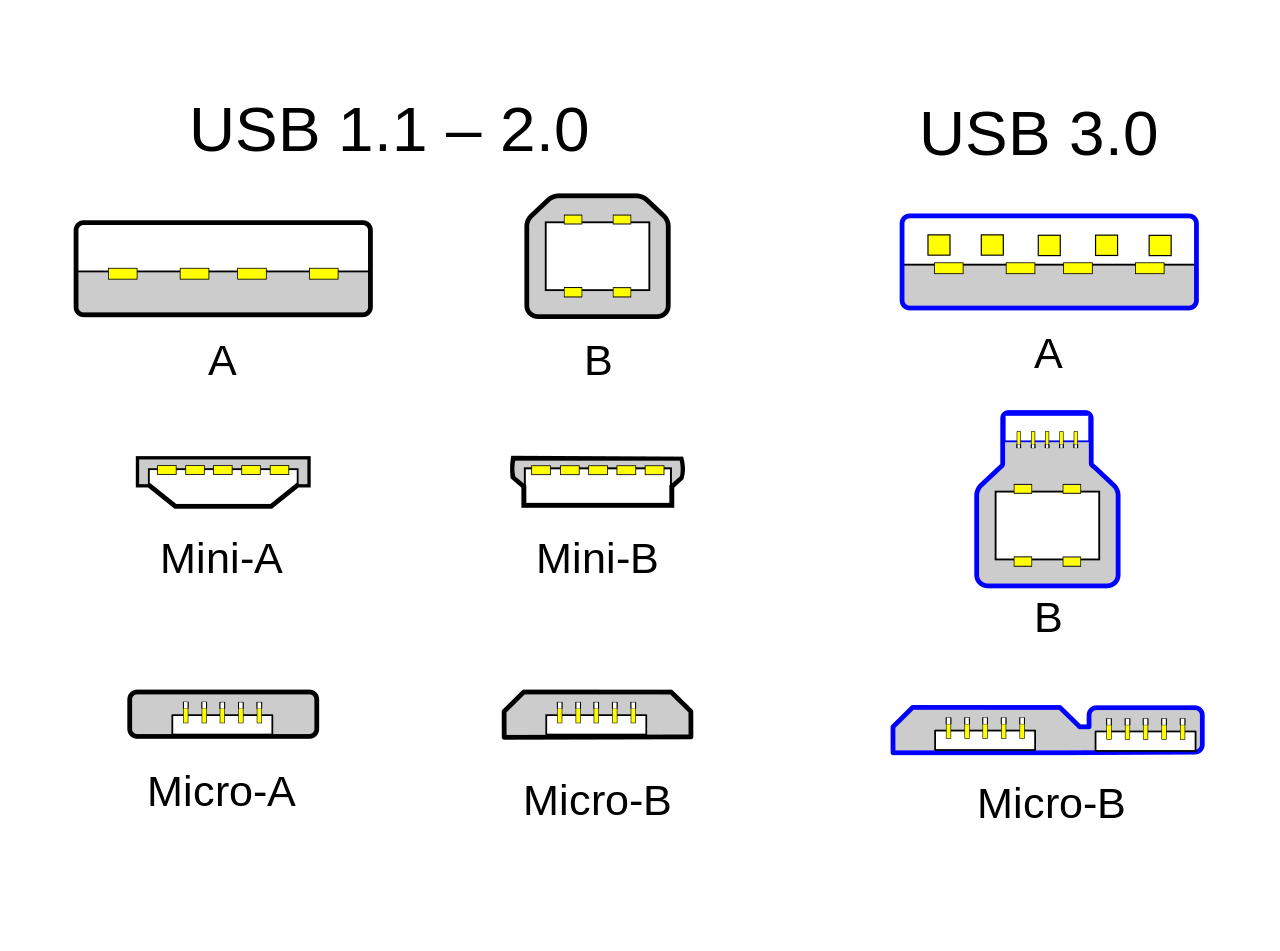
\includegraphics[width=0.6\textwidth]{images/usb_connectors.png}
    \caption{Connectors USB de tipus A i B. \cite{Contributors2024USB}}
    \label{fig:usb_connectors}
\end{figure}

\begin{itemize}
    \item Els connectors de tiups A son els que es connecten al dispositiu
    que actuarà com a mestre. Existeixen les variants \est{micro} i \est{mini},
    com es pot observar a la Figura \ref{fig:usb_connectors}, tot i que aquestes
    so son gaire populars. Amb l'aparició de l'estàndard \acro{usb3}, es van
    dissenyar nous connectors que fóssin compatibles amb els dels estàndards
    anteriors.
    \item Els connectors de tipus B son els que es connecten a l'esclau. Aquests
    també tenen les variants \est{micro} i \est{mini}, molt utilitzades
    en l'electrònica domèstica. També es va crear nous connectors de tipus B
    per a poder acollir l'estàndard \acro{usb3}.
    \item Finalment, els connectors de tipus C no tenen una jerarquia definida:
    serveixen per a dispositius que poden ser mestres o esclaus en diferents
    moments donats. La decisió de qui actua de mestre es pacta just a l'inici
    de la connexió, mitjançant un protocol específic \cite{Axelson2015USB}.
    Aquest connector, a diferència de la reta, és reversible: es pot connectar
    en les dues orientacions possibles. Es pot veure l'aspecte del connector
    a la Figura \ref{fig:usb_connectors_c}.
\end{itemize}

\begin{figure}[ht]
    \centering
    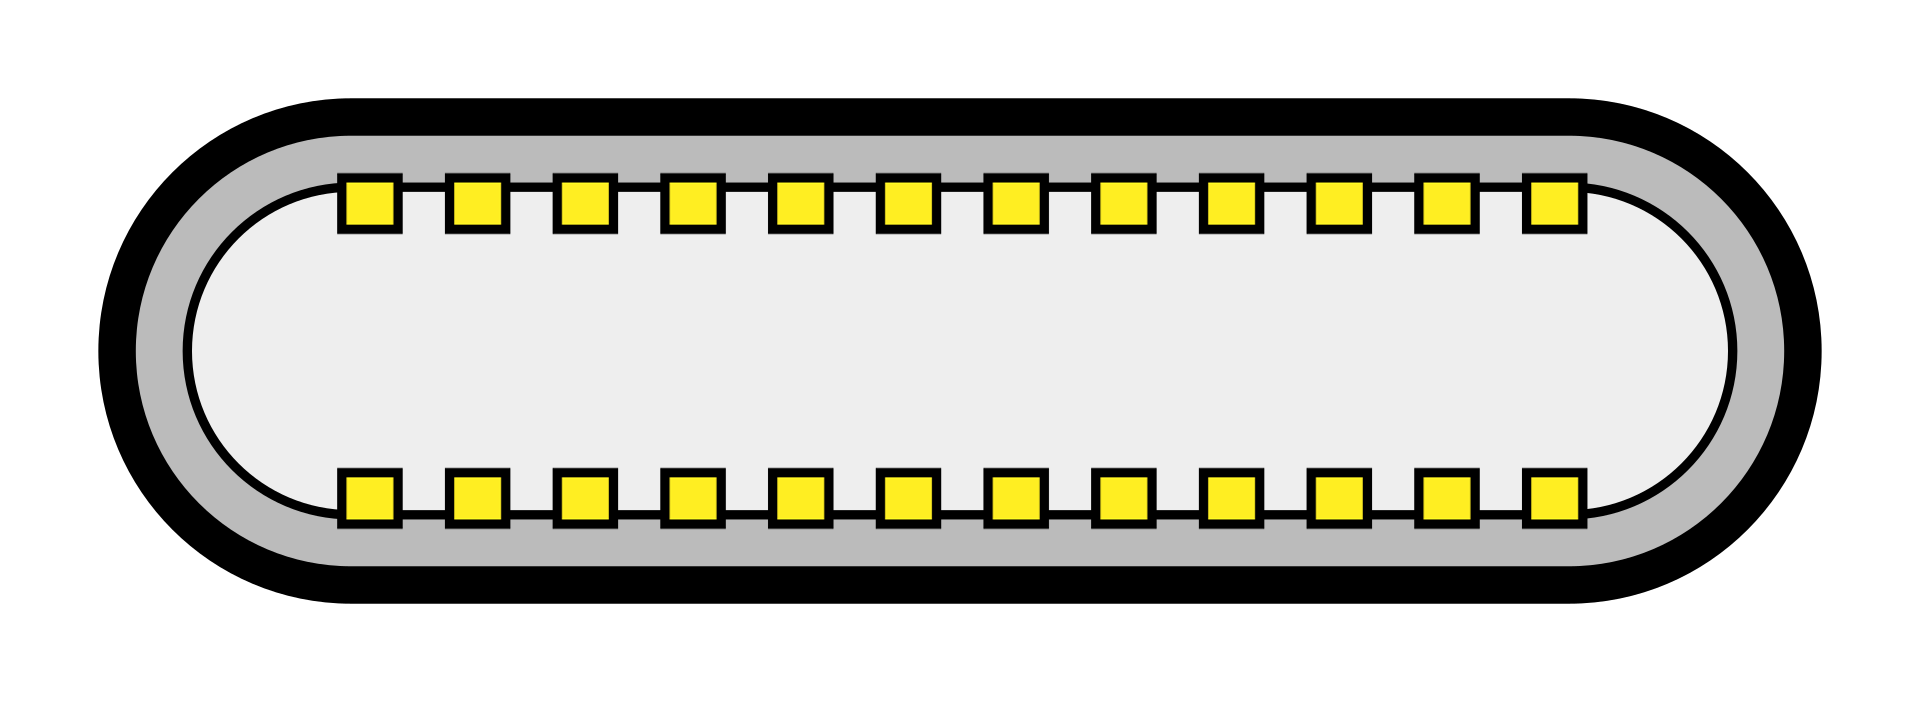
\includegraphics[width=0.3\textwidth]{images/usb_c.png}
    \caption{Connector USB de tipus C. \cite{Contributors2024USB}}
    \label{fig:usb_connectors_c}
\end{figure}

Així doncs, gairebé la totalitat de cables \acro{usb} seran de tipus A a tipus
B, utilitzant qualsevol format de mida. El tipus C, al ser bidireccional, pot
substituir el tipus A o el tipus B en els cables mencionats anteriorment.
Quan un cable només té un connector de tipus C en un cantó, no s'ha de pactar
la jerarquia de mestre-esclau, ja que ve definida pel tipus de connector a
l'altra banda del cable. Evidentment, també hi pot haver cables de tipus C a
tipus C.

Tanmateix, a l'any 2022 el Consell de la Unió Europea va aprovar una llei
que obliga un seguit de dispositius electrònics a utilitzar el connector
\acro{usb-c} enlloc d'altres estàndards \cite{Council2022Common}. Segons la
nota de premsa, el motiu d'aquesta llei és per a evitar més deixalla electrònica
per culpa de tenir diferents dispositius amb diferents connectors, així com
facilitar l'ús de les tecnologies als consumidors. Aquesta llei
es començarà a aplicar a finals de l'any 2024, i afectarà dispositius mòbils, 
alguns portàtils, tauletes, teclats i ratolins ina\l.làmbrics, entre
d'altres.

Sent el dispositu que es vol crear en aquest projecte un perifèric de
l'ordinador, la llei citada no l'afectaria. Tanmateix, la mateixa nota de premsa
informa sobre la intenció d'extendre aquest connector a altres dispositius.
Tenint present que el dispositiu que es vol crear podria entrar fàcilment en
aquest grup de perifèrics d'ordinador, s'ha decidit utilitzar un connector de
tipus \acro{usb-c} per a assegurar-nos la seva possible comercialització dintre
de la UE.


\chapter{Hardware}
\chapter{Firmware}
\chapter{software}

\chapter{Estudi econòmic}
\chapter{Conclusions}
\chapter{Treball futur}


\printbibliography

%\appendix
%\part{Apèndixs}
%\chapter{Un apèndix}

\end{document}

%%% Local Variables:
%%% mode: latex
%%% TeX-master: t
%%% LaTeX-biblatex-use-Biber: t
%%% End:
